%**************************************%
%* Generated from MathBook XML source *%
%*    on 2016-06-29T13:04:48-04:00    *%
%*                                    *%
%*   http://mathbook.pugetsound.edu   *%
%*                                    *%
%**************************************%
\documentclass[10pt,]{book}
%% Load geometry package to allow page margin adjustments
\usepackage{geometry}
\geometry{letterpaper,total={5.0in,9.0in}}
%% Custom Preamble Entries, early (use latex.preamble.early)
%% Inline math delimiters, \(, \), need to be robust
%% 2016-01-31:  latexrelease.sty  supersedes  fixltx2e.sty
%% If  latexrelease.sty  exists, bugfix is in kernel
%% If not, bugfix is in  fixltx2e.sty
%% See:  https://tug.org/TUGboat/tb36-3/tb114ltnews22.pdf
%% and read "Fewer fragile commands" in distribution's  latexchanges.pdf
\IfFileExists{latexrelease.sty}{}{\usepackage{fixltx2e}}
%% Page Layout Adjustments (latex.geometry)
%% For unicode character support, use the "xelatex" executable
%% If never using xelatex, the next three lines can be removed
\usepackage{ifxetex}
\ifxetex\usepackage{xltxtra}\fi
%% Symbols, align environment, bracket-matrix
\usepackage{amsmath}
\usepackage{amssymb}
%% allow more columns to a matrix
%% can make this even bigger by overriding with  latex.preamble.late  processing option
\setcounter{MaxMatrixCols}{30}
%% Semantic Macros
%% To preserve meaning in a LaTeX file
%% Only defined here if required in this document
%% Used for inline definitions of terms
\newcommand{\terminology}[1]{\textbf{#1}}
%% Subdivision Numbering, Chapters, Sections, Subsections, etc
%% Subdivision numbers may be turned off at some level ("depth")
%% A section *always* has depth 1, contrary to us counting from the document root
%% The latex default is 3.  If a larger number is present here, then
%% removing this command may make some cross-references ambiguous
%% The precursor variable $numbering-maxlevel is checked for consistency in the common XSL file
\setcounter{secnumdepth}{3}
%% Environments with amsthm package
%% Theorem-like environments in "plain" style, with or without proof
\usepackage{amsthm}
\theoremstyle{plain}
%% Numbering for Theorems, Conjectures, Examples, Figures, etc
%% Controlled by  numbering.theorems.level  processing parameter
%% Always need a theorem environment to set base numbering scheme
%% even if document has no theorems (but has other environments)
\newtheorem{theorem}{Theorem}[section]
%% Only variants actually used in document appear here
%% Style is like a theorem, and for statements without proofs
%% Numbering: all theorem-like numbered consecutively
%% i.e. Corollary 4.3 follows Theorem 4.2
%% Definition-like environments, normal text
%% Numbering is in sync with theorems, etc
\theoremstyle{definition}
\newtheorem{definition}[theorem]{Definition}
%% Example-like environments, normal text
%% Numbering is in sync with theorems, etc
\theoremstyle{definition}
\newtheorem{example}[theorem]{Example}
%% Miscellaneous environments, normal text
%% Numbering for inline exercises and lists is in sync with theorems, etc
\theoremstyle{definition}
\newtheorem{exercise}[theorem]{Exercise}
%% Localize LaTeX supplied names (possibly none)
\renewcommand*{\chaptername}{Chapter}
%% For improved tables
\usepackage{array}
%% Some extra height on each row is desirable, especially with horizontal rules
%% Increment determined experimentally
\setlength{\extrarowheight}{0.2ex}
%% Define variable thickness horizontal rules, full and partial
%% Thicknesses are 0.03, 0.05, 0.08 in the  booktabs  package
\makeatletter
\newcommand{\hrulethin}  {\noalign{\hrule height 0.04em}}
\newcommand{\hrulemedium}{\noalign{\hrule height 0.07em}}
\newcommand{\hrulethick} {\noalign{\hrule height 0.11em}}
%% We preserve a copy of the \setlength package before other
%% packages (extpfeil) get a chance to load packages that redefine it
\let\oldsetlength\setlength
\newlength{\Oldarrayrulewidth}
\newcommand{\crulethin}[1]%
{\noalign{\global\oldsetlength{\Oldarrayrulewidth}{\arrayrulewidth}}%
\noalign{\global\oldsetlength{\arrayrulewidth}{0.04em}}\cline{#1}%
\noalign{\global\oldsetlength{\arrayrulewidth}{\Oldarrayrulewidth}}}%
\newcommand{\crulemedium}[1]%
{\noalign{\global\oldsetlength{\Oldarrayrulewidth}{\arrayrulewidth}}%
\noalign{\global\oldsetlength{\arrayrulewidth}{0.07em}}\cline{#1}%
\noalign{\global\oldsetlength{\arrayrulewidth}{\Oldarrayrulewidth}}}
\newcommand{\crulethick}[1]%
{\noalign{\global\oldsetlength{\Oldarrayrulewidth}{\arrayrulewidth}}%
\noalign{\global\oldsetlength{\arrayrulewidth}{0.11em}}\cline{#1}%
\noalign{\global\oldsetlength{\arrayrulewidth}{\Oldarrayrulewidth}}}
%% Single letter column specifiers defined via array package
\newcolumntype{A}{!{\vrule width 0.04em}}
\newcolumntype{B}{!{\vrule width 0.07em}}
\newcolumntype{C}{!{\vrule width 0.11em}}
\makeatother
%% Figures, Tables, Listings, Floats
%% The [H]ere option of the float package fixes floats in-place,
%% in deference to web usage, where floats are totally irrelevant
%% We re/define the figure, table and listing environments, if used
%%   1) New mbxfigure and/or mbxtable environments are defined with float package
%%   2) Standard LaTeX environments redefined to use new environments
%%   3) Standard LaTeX environments redefined to step theorem counter
%%   4) Counter for new environments is set to the theorem counter before caption
%% You can remove all this figure/table setup, to restore standard LaTeX behavior
%% HOWEVER, numbering of figures/tables AND theorems/examples/remarks, etc
%% WILL ALL de-synchronize with the numbering in the HTML version
%% You can remove the [H] argument of the \newfloat command, to allow flotation and 
%% preserve numbering, BUT the numbering may then appear "out-of-order"
\usepackage{float}
\usepackage[bf]{caption} % http://tex.stackexchange.com/questions/95631/defining-a-new-type-of-floating-environment 
\usepackage{newfloat}
% Figure environment setup so that it no longer floats
\SetupFloatingEnvironment{figure}{fileext=lof,placement={H},within=section,name=Figure}
% figures have the same number as theorems: http://tex.stackexchange.com/questions/16195/how-to-make-equations-figures-and-theorems-use-the-same-numbering-scheme 
\makeatletter
\let\c@figure\c@theorem
\makeatother
% Table environment setup so that it no longer floats
\SetupFloatingEnvironment{table}{fileext=lot,placement={H},within=section,name=Table}
% tables have the same number as theorems: http://tex.stackexchange.com/questions/16195/how-to-make-equations-figures-and-theorems-use-the-same-numbering-scheme 
\makeatletter
\let\c@table\c@theorem
\makeatother
%% Raster graphics inclusion, wrapped figures in paragraphs
\usepackage{graphicx}
%% Colors for Sage boxes and author tools (red hilites)
\usepackage[usenames,dvipsnames,svgnames,table]{xcolor}
%% New typewriter font if  c, sage, program, console, pre  tags present
%% If only  email, url  tags, no change from default
%% Needs a bit of scaling down to match text
\usepackage[scaled=.95]{sourcecodepro}
%% Program listing support, for inline code, Sage code
\usepackage{listings}
%% We define the listings font style to be the default "ttfamily"
%% To fix hyphens/dashes rendered in PDF as fancy minus signs by listing
%% http://tex.stackexchange.com/questions/33185/listings-package-changes-hyphens-to-minus-signs
\makeatletter
\lst@CCPutMacro\lst@ProcessOther {"2D}{\lst@ttfamily{-{}}{-{}}}
\@empty\z@\@empty
\makeatother
%% End of generic listing adjustments
%% Inline code, typically from "c" element
%% Global, document-wide options apply to \lstinline
%% Search/replace \lstinline by \verb to remove this dependency
%% (redefining \lstinline with \verb is unlikely to work)
%% Also see "\renewcommand\UrlFont" below for matching font choice
\lstset{basicstyle=\small\ttfamily,breaklines=true,breakatwhitespace=true}
%% More flexible list management, esp. for references and exercises
%% But also for specifying labels (i.e. custom order) on nested lists
\usepackage{enumitem}
%% hyperref driver does not need to be specified
\usepackage{hyperref}
%% Hyperlinking active in PDFs, all links solid and blue
\hypersetup{colorlinks=true,linkcolor=blue,citecolor=blue,filecolor=blue,urlcolor=blue}
\hypersetup{pdftitle={Test chapter}}
%% If you manually remove hyperref, leave in this next command
\providecommand\phantomsection{}
%% Use upright quotes rather than LaTeX's curly quotes
%% If custom font substitutions follow, this might be ineffective
%% If fonts lack upright quotes, the textcomp package is employed
\usepackage{upquote}
%% Graphics Preamble Entries
\usepackage{pgfplots}               % loads tikz package
\pgfplotsset{axis x line = middle,
             axis y line = middle}
\usetikzlibrary{backgrounds}
\usetikzlibrary{arrows,matrix}
%% If tikz has been loaded, replace ampersand with \amp macro
%% extpfeil package for certain extensible arrows,
%% as also provided by MathJax extension of the same name
%% NB: this package loads mtools, which loads calc, which redefines
%%     \setlength, so it can be removed if it seems to be in the 
%%     way and your math does not use:
%%     
%%     \xtwoheadrightarrow, \xtwoheadleftarrow, \xmapsto, \xlongequal, \xtofrom
%%     
%%     we have had to be extra careful with variable thickness
%%     lines in tables, and so also load this package late
\usepackage{extpfeil}
%% Custom Preamble Entries, late (use latex.preamble.late)
%% Begin: Author-provided macros
%% (From  docinfo/macros  element)
%% Plus three from MBX for XML characters
\newcommand{\alert}[1]{\mathbf{\color{magenta}{#1}}}
\delimitershortfall-1sp
\newcommand\abs[1]{\left|#1\right|}

\newcommand\degree[0]{^{\circ}}
\newcommand{\lt}{ < }
\newcommand{\gt}{ > }
\newcommand{\amp}{ & }
%% End: Author-provided macros
%% Title page information for book
\title{Test chapter\\
{\large test subtitle}}
\author{}
\date{}
\begin{document}
\typeout{************************************************}
\typeout{Chapter 1 Fake chapter}
\typeout{************************************************}
\chapter[Fake chapter]{Fake chapter}\label{testchap}
\typeout{************************************************}
\typeout{Introduction  }
\typeout{************************************************}
\typeout{************************************************}
\typeout{Section 1.1 Logarithms}
\typeout{************************************************}
\section[Logarithms]{Logarithms}\label{Logarithms}

	In this section, we introduce a new mathematical tool called a \emph{logarithm}, which will help us solve exponential equations.
%
\par

	Suppose that a colony of bacteria doubles in size every day. If the colony starts with \(50\) bacteria, how long will it be before there are \(800\) bacteria? We answered questions of this type in {$\langle\langle$Unresolved xref, reference "Exponential-Functions"; check spelling or use "provisional" attribute$\rangle\rangle$} by writing and solving an exponential equation. The function
	\begin{equation*}P(t) = 50 \cdot 2^t\end{equation*}
	gives the number of bacteria present on day \(t\), so we must solve the equation
	\begin{equation*}800 = 50 \cdot 2^t\end{equation*}
	Dividing both sides by 50 yields
	\begin{equation*}16 = 2^t\end{equation*}
	The solution of this equation is the answer to the following question: To what power must we raise \(2\) in order to get \(16\)?
%
\par

	The value of \(t\) that solves the equation is called the base \(2\) \terminology{logarithm} of \(16\). Since \(2^4 = 16\), the base \(2\) logarithm of \(16\) is \(4\). We write this as
	\begin{equation*}\log_{2}16 = 4\end{equation*}
	In other words, we solve an exponential equation by computing a logarithm. You can check that \(t = \alert{4}\)
	solves the problem stated above:
	\begin{equation*}P(\alert{4}) = 50 \cdot 2^\alert{4}= 800\end{equation*}
%
\par

	Thus, the unknown exponent is called a logarithm. In general, for positive values of \(b\) and \(x\), we make the following definition.
%
\begin{definition}[Logarithm]\label{definition-1}

	The \terminology{base \(b\) logarithm of \(x\)}, written \(\log_{b} x\), is the exponent to which \(b\) must be raised in order to yield \(x\).
\end{definition}
\par

	It will help to keep in mind that a logarithm is just an exponent. Some logarithms, like some square roots, are easy to evaluate, while others require a calculator. We will start with the easy ones.
%
\begin{example}[]\label{example-easy-logarithm}

	Compute the logarithms.
	\leavevmode%
\begin{enumerate}[label=*\alph**]
\item\hypertarget{li-1}{}\(\log_3 9\)\item\hypertarget{li-2}{}\(\log_5 125 \)\item\hypertarget{li-3}{}\(\log_4 \frac{1}{16}\)\item\hypertarget{li-4}{}\(\log_5 \sqrt{5}\)\end{enumerate}

%
\par\medskip\noindent%
\textbf{Solution.}\quad \leavevmode%
\begin{enumerate}[label=*\alph**]
\item\hypertarget{li-5}{}
		To evaluate \(\log_3 9\), we ask what exponent on base \(3\) will produce \(9\). In symbols, we want to fill in the blank in the equation \(3^{\underline{?}} = 9\). The exponent we need is \(2\), so
		\begin{equation*}\log_3 9 = 2 \text{ because } 3^2 = 9\end{equation*}
		We use similar reasoning to compute the other logarithms.
	\item\hypertarget{li-6}{}\(\log_5{125} = 3 \text{ because } 5^3 = 125\)\item\hypertarget{li-7}{}\(\log_4{\frac{1}{16}}= −2 \text{ because } 4^{−2} = \frac{1}{16}\)\item\hypertarget{li-8}{}\(\log_5{\sqrt{5}} = \frac{1}{2} \text{ because } 5^{1/2} =\sqrt{5}\)\end{enumerate}
\end{example}
\begin{exercise}\label{exercise-easy-logarithms}

	Find each logarithm.
	\leavevmode%
\begin{enumerate}[label=*\alph**]
\item\hypertarget{li-9}{}\(\log_{3}{81}\)\item\hypertarget{li-10}{}\(\log_{10}{\frac{1}{1000}}\)\end{enumerate}
\end{exercise}
\par

	From the definition of a logarithm and the examples above, we see that the following two statements are equivalent.
%
\typeout{************************************************}
\typeout{Paragraphs  Logarithms and Exponents: Conversion Equations}
\typeout{************************************************}
\paragraph[Logarithms and Exponents: Conversion Equations]{Logarithms and Exponents: Conversion Equations}\label{paragraphs-1}

	If \(b \gt 0\) and \(x \gt 0\),
	\begin{equation*}y = \log_b x \text{ if and only if } x = b^y\end{equation*}
%
\par

	In other words, the logarithm \(y\), is the same as the \emph{exponent} in \(x = b^y\). We see again that \emph{a logarithm is an exponent}; it is the exponent to which \(b\) must be raised to yield \(x\).
%
\par

	These equations allow us to convert from logarithmic to exponential form, or vice versa. You should memorize the conversion equations, because we will use them frequently. 
%
\par

	As special cases of the equivalence in (1), we can compute the following useful logarithms.
For any base \(b \gt 0\),
%
\typeout{************************************************}
\typeout{Paragraphs  Some Useful Logarithms}
\typeout{************************************************}
\paragraph[Some Useful Logarithms]{Some Useful Logarithms}\label{paragraphs-2}

	\begin{align*}
	\log_b b \amp = 1 \text{ because } b^1 = b \\
	\log_b 1 \amp = 0  \text{ because } b^0 = 1 \\
	\log_b{bx} \amp = x \text{ because } b^x = b^x
	\end{align*}
%
\begin{example}[]\label{example-useful-logarithms}
\leavevmode%
\begin{enumerate}[label=*\alph**]
\item\hypertarget{li-11}{}\(\log_{2}{2} = 1\)\item\hypertarget{li-12}{}\(\log_{5}{1} = 0\)\item\hypertarget{li-13}{}\(\log_{3}{3^4} = 4\)\end{enumerate}
\end{example}
\begin{exercise}\label{exercise-useful-logarithms}

	Find each logarithm.
	\leavevmode%
\begin{enumerate}[label=*\alph**]
\item\hypertarget{li-14}{}\(\log_{n}{1}\)\item\hypertarget{li-15}{}\(\log_{n}{n^3}\)\end{enumerate}
\end{exercise}
\typeout{************************************************}
\typeout{Subsection 1.1.1 Using the Conversion Equations}
\typeout{************************************************}
\subsection[Using the Conversion Equations]{Using the Conversion Equations}\label{subsection-1}

	We use logarithms to solve exponential equations, just as we use square roots to solve quadratic equations. Consider the two equations
	\begin{equation*}x^2 = 25 ~ \text{ and } ~ 2^x = 8\end{equation*}
	We solve the first equation by taking a square root, and we solve the second equation by computing a logarithm:
	\begin{equation*}x = \pm\sqrt{25} = \pm 5 ~ \text{ and } ~ x = \log_{2}{8} = 3\end{equation*}
	The operation of taking a base \(b\) logarithm is the inverse operation for raising the base \(b\) to a power, just as extracting square roots is the inverse of squaring a number.
%
\par

	Every exponential equation can be rewritten in logarithmic form by using the conversion equations. Thus,
	\begin{equation*}3 = \log_{2}{8} \text{ and } 8 = 2^3\end{equation*}
	are equivalent statements, just as
	\begin{equation*}5 = \sqrt{25} \text{ and } 25 = 5^2\end{equation*}
	are equivalent statements. Rewriting an equation in logarithmic form is a basic  strategy for finding its solution.
%
\begin{example}[]\label{example-exponential-to-log-form}

	Rewrite each equation in logarithmic form.
	\leavevmode%
\begin{enumerate}[label=*\alph**]
\item\hypertarget{li-16}{}\(2^{−1} = \frac{1}{2}\)\item\hypertarget{li-17}{}\(a^{1/5} = 2.8\)\item\hypertarget{li-18}{}\(6^{1.5} = T\)\item\hypertarget{li-19}{}\(M^v = 3K\)\end{enumerate}

%
\par\medskip\noindent%
\textbf{Solution.}\quad 
	First identify the base \(b\), and then the exponent or logarithm \(y\). Use the conversion equations to rewrite \(b^y = x\) in the form \(\log_{b}{x} = y\).
	\leavevmode%
\begin{enumerate}[label=*\alph**]
\item\hypertarget{li-20}{}The base is \(2\) and the exponent is \(−1\). Thus, \(\log_{2}{\frac{1}{2}}= −1\).\item\hypertarget{li-21}{}The base is \(a\) and the exponent is \(\frac{1}{5}\). Thus, \(\log_{a}{2.8} = \frac{1}{5}\).\item\hypertarget{li-22}{}The base is \(6\) and the exponent is \(1.5\). Thus, \(\log_{6}{T} = 1.5\).\item\hypertarget{li-23}{}The base is \(M\) and the exponent is \(v\). Thus, \(\log_{M}{3K} = v\).\end{enumerate}

%
\end{example}
\begin{exercise}\label{exercise-exponential-to-log-form}

	Rewrite each equation in logarithmic form.
	\leavevmode%
\begin{enumerate}[label=*\alph**]
\item\hypertarget{li-24}{}\(8^{−1/3} = \frac{1}{2}\)\item\hypertarget{li-25}{}\(5^x = 46\)\end{enumerate}

%
\end{exercise}
\typeout{************************************************}
\typeout{Subsection 1.1.2 Approximating Logarithms}
\typeout{************************************************}
\subsection[Approximating Logarithms]{Approximating Logarithms}\label{subsection-2}

	Suppose we would like to solve the equation
	\begin{equation*}2^x = 26\end{equation*}
	The solution of this equation is \(x = \log_{2}{26}\), but can we find a decimal approximation for this value? There is no integer power of \(2\) that equals \(26\), because
	\begin{align*}
	2^4 \amp = 16 \\
	\text{and } 2^5 \amp = 32
	\end{align*} 
	Thus, \(\log_{2}{26}\) must be between \(4\) and \(5\). We can use trial and error to find the value of \(\log_{2}{26}\) to the nearest tenth. Use your calculator to make a table of values for \(y = 2^x\), starting with \(x = 4\) and using increments of \(0.1\).
%
\leavevmode%
\begin{table}
\centering
\begin{tabular}{AcAcAcAcAcA}\crulethin{1-2}\crulethin{4-5}
\(x\)&\(2^x\)&&\(x\)&\(2^x\)\tabularnewline\crulethick{1-2}\crulethick{4-5}
\(4\)&\(2^4=16\)&&\(4.5\)&\(2^{4.5}=22.627\)\tabularnewline\crulethin{1-2}\crulethin{4-5}
\(4.1\)&\(2^{4.1}=17.148\)&&\(4.6\)&\(2^{4.6}=24.251\)\tabularnewline\crulethin{1-2}\crulethin{4-5}
\(4.2\)&\(2^{4.2}=18.379\)&&\(\alert{4.7}\)&\(2^{\alert{4.7}}=25.992\)\tabularnewline\crulethin{1-2}\crulethin{4-5}
\(4.3\)&\(2^{4.3}=19.698\)&&\(\alert{4.8}\)&\(2^{\alert{4.8}}=27.858\)\tabularnewline\crulethin{1-2}\crulethin{4-5}
\(4.4\)&\(2^{4.4}=21.112\)&&\(4.9\)&\(2^{4.9}=29.857\)\tabularnewline\crulethin{1-2}\crulethin{4-5}
\end{tabular}
\caption{\label{table-decimal-powers-of-two}}
\end{table}
\par

	From \hyperref[table-decimal-powers-of-two]{Table~\ref{table-decimal-powers-of-two}}, we see that \(26\) is between \(24.7\) and \(24.8\), and is closer to \(24.7\). To the nearest tenth, \(\log_{2}{26} \approx 4.7\).
%
\par

	Trial and error can be a time-consuming process. In Example 4, we illustrate a graphical method for estimating the value of a logarithm.
%
\begin{example}[]\label{example-approximate-log}

	Approximate \(\log_{3}{7}\) to the nearest hundredth.
%
\par\medskip\noindent%
\textbf{Solution.}\quad 
	If \(\log_{3}{7}=x\), then \(3^x = 7\). We will use the graph of \(y = 3^x\) to approximate a solution to \(3^x = 7\). Graph \(Y_1 =3\)\lstinline?^? X and \(Y_2 = 7\) in the standard window (\lstinline?ZOOM? 6) to obtain the graph shown in \hyperref[fig-GC-approx-log]{Figure~\ref{fig-GC-approx-log}}. Activate the intersect feature to find that the two graphs intersect at the point \((1.7712437, 7)\). Because this point lies on the graph of \(y = 3^x\) , we know that
	\begin{equation*}31.7712437 \approx 7\text{, or } \log_{3}{7} \approx 1.7712437\end{equation*}
	To the nearest hundredth, \(\log_{3}{7} \approx 1.77\).
%
\leavevmode%
\begin{figure}
\centering
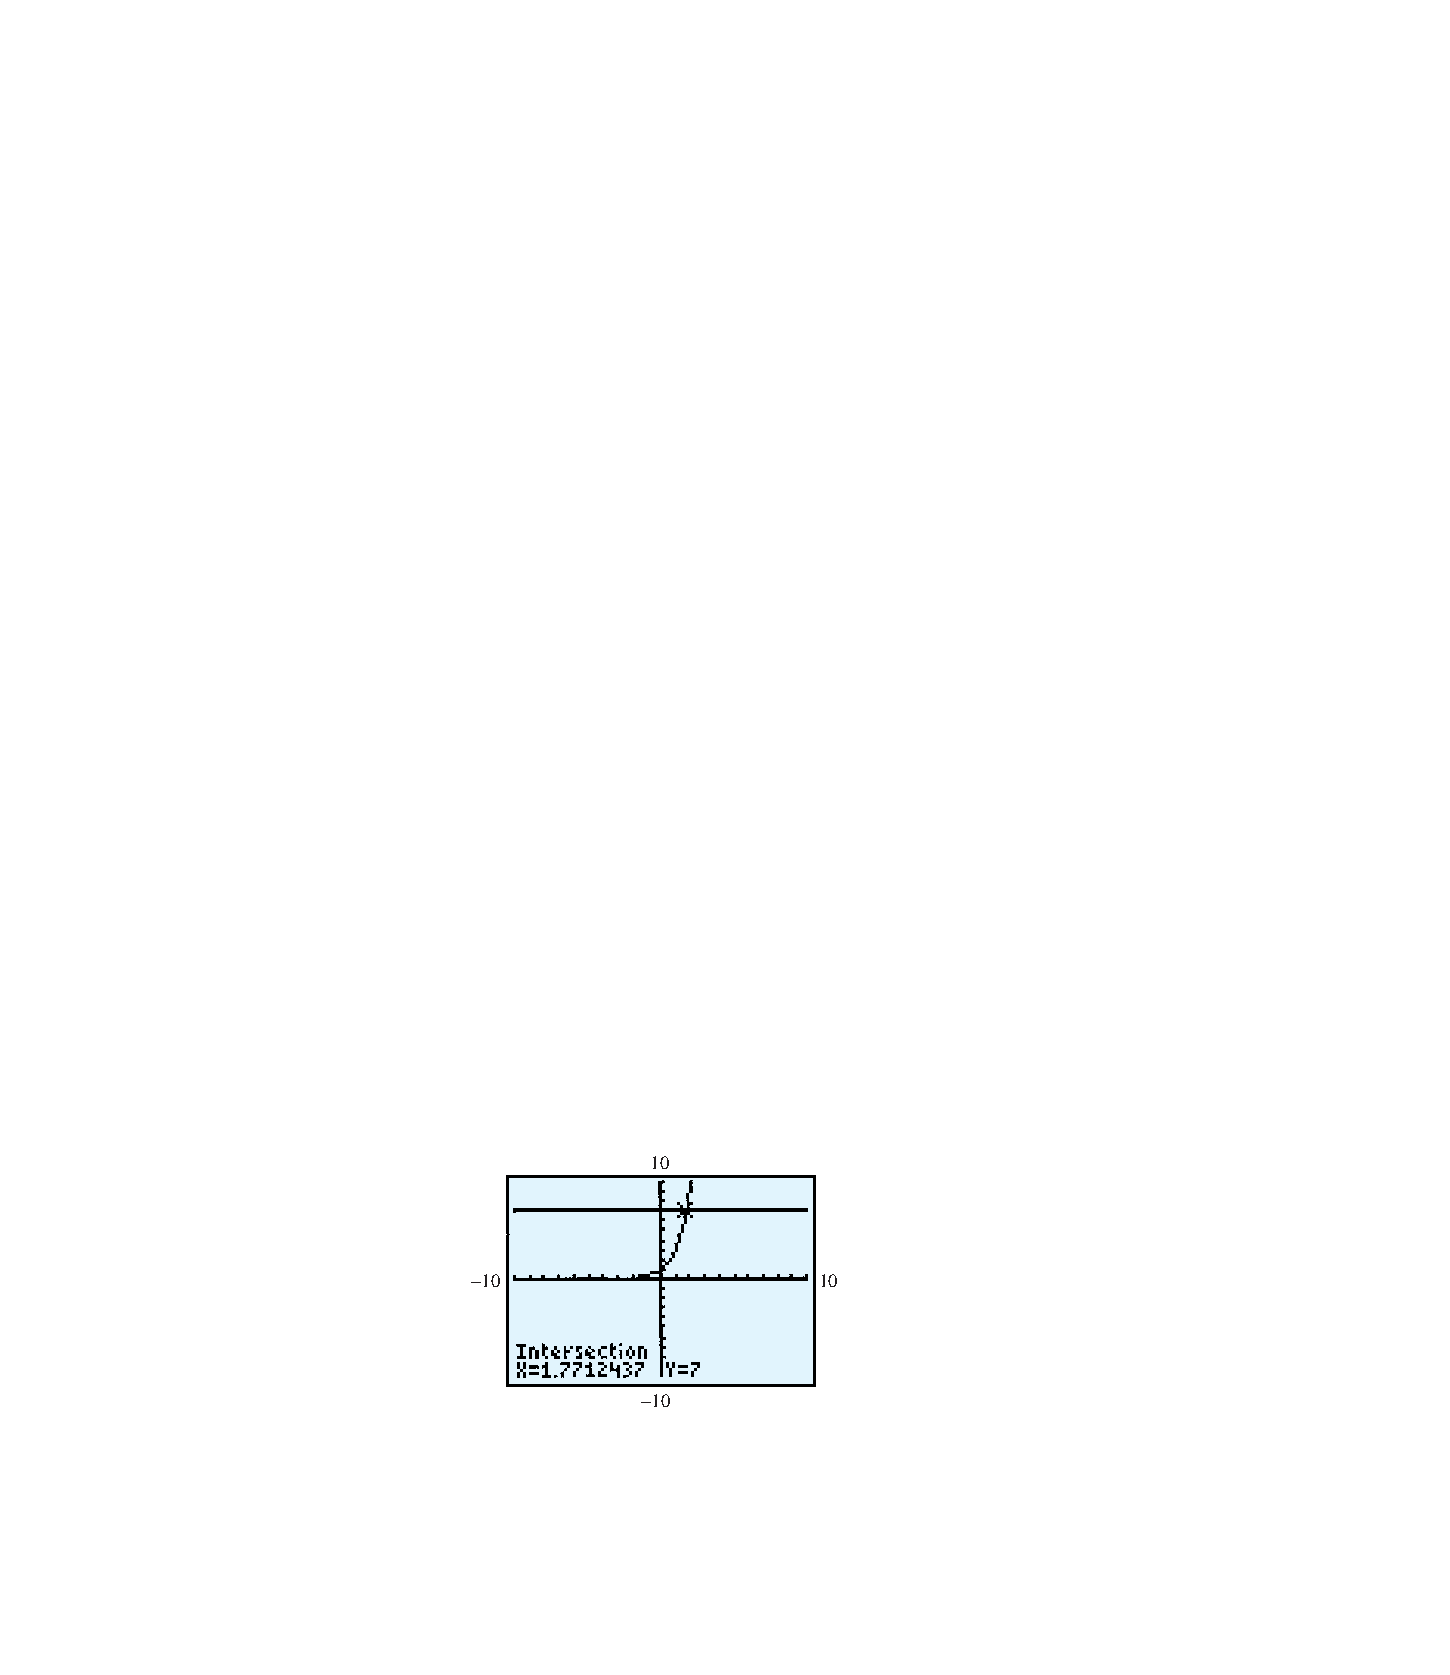
\includegraphics[width=0.60\textwidth,]{images/fig-GC-approx-log.pdf}\caption{\label{fig-GC-approx-log}}
\end{figure}
\end{example}
\begin{exercise}\label{exercise-approximate-log}
\leavevmode%
\begin{enumerate}[label=*\alph**]
\item\hypertarget{li-26}{}Rewrite the equation \(3^x = 90\) in logarithmic form.\item\hypertarget{li-27}{}Use a graph to approximate the solution to the equation in part (a). Round your answer to three decimal places.\end{enumerate}
\end{exercise}
\typeout{************************************************}
\typeout{Subsection 1.1.3 Base 10 Logarithms}
\typeout{************************************************}
\subsection[Base 10 Logarithms]{Base 10 Logarithms}\label{subsection-3}

	Some logarithms are used so frequently in applications that their values are programmed into scientific and graphing calculators. These are the base \(10\) logarithms, such as 
	\begin{equation*}\log_{10}{1000} = 3 ~\text{ and }~ \log_{10}{0.01} = −2\end{equation*}
	Base \(10\) logarithms are called \terminology{common logarithms}, and the subscript \(10\) is often omitted, so that \(\log x\) is understood to mean \(\log_{10}{x}\).
%
\par

	To evaluate a base \(10\) logarithm, we use the \lstinline?LOG? key on a calculator. Many logarithms are irrational numbers, and the calculator gives as many digits as its display allows. We can then round off to the desired accuracy.
%
%
%% The index is here, setup is all in preamble
\printindex
%
This book was authored in MathBook XML.%
\end{document}